% =============================================================
%  PDC Assignment 2 -- StudySync Resilience Report
%  Author:  Aqib Bin Qamar (BSCS23178)
%  Compile: pdflatex report.tex   (Overleaf works out of the box)
% =============================================================
\documentclass[11pt]{article}

\usepackage[a4paper, margin=0.85in]{geometry}
\usepackage{microtype}
\usepackage{enumitem}
\usepackage{booktabs}
\usepackage{xcolor}
\usepackage{listings}
\usepackage{tikz}
\usetikzlibrary{positioning, arrows.meta, calc, fit}
\usepackage{titlesec}
\usepackage{parskip}

\titlespacing*{\section}{0pt}{1.0ex plus .2ex}{0.6ex plus .1ex}
\titlespacing*{\subsection}{0pt}{0.7ex plus .2ex}{0.4ex plus .1ex}
\setlist{nosep, leftmargin=1.3em}

\lstdefinestyle{sql}{
  basicstyle=\ttfamily\footnotesize,
  keywordstyle=\bfseries,
  language=SQL, frame=single, framesep=3pt, rulecolor=\color{gray!40},
  showstringspaces=false, breaklines=true, columns=fullflexible,
  aboveskip=2pt, belowskip=2pt
}

\title{\vspace{-2em}\textbf{Building Resilient Distributed Systems --- StudySync}}
\author{Aqib Bin Qamar \quad (BSCS23178) \\ \small Parallel and Distributed Computing}
\date{\vspace{-0.8em}}

\begin{document}
\maketitle
\vspace{-2.0em}

% =============================================================
\section*{Part 1 --- Analysis}

\subsection*{1.1 Synchronization: the Lost Update on shared documents}
The naive flow is \texttt{GET /doc/:id} $\rightarrow$ user edits in React $\rightarrow$ \texttt{PUT /doc/:id}, with a single
\texttt{UPDATE documents SET body=:b WHERE id=:id} on the backend. There is no version or timestamp predicate, so
when two users both read revision 7 and both \texttt{PUT}, the second write unconditionally overwrites the first. This is the
textbook \textbf{Lost Update} anomaly: the database has no information about which revision each client based its edit on,
so it cannot reject the stale write. SQLAlchemy session isolation does not save us --- both transactions are internally
consistent and commit successfully; the conflict is \emph{between} transactions and lives at the application layer.

\subsection*{1.2 Coordination: a dropped Clerk webhook = permanent inconsistency}
Clerk sends \texttt{subscription.deleted} over HTTP, fire-and-forget. The backend handles it inline, mutates
\texttt{users.is\_premium=false}, and returns 200. Three failures break this:
\begin{itemize}
  \item \textbf{Network blip} --- Clerk's POST never reaches us; Clerk retries a few times then gives up.
  \item \textbf{Crash mid-handler} --- the row is updated but the response is lost; Clerk retries, the handler runs
  again, and any non-idempotent side effect (e.g. a refund) happens twice.
  \item \textbf{Out-of-order delivery} --- a later \texttt{subscription.created} arrives before the original
  \texttt{deleted}, leaving the user premium forever.
\end{itemize}
The root cause is treating an \emph{at-least-once} delivery channel as if it were \emph{exactly-once}: there is no
idempotency key, no durable inbox, no retry queue, and no DLQ. A single dropped event permanently desyncs Clerk
from our database.

\subsection*{1.3 Fault Tolerance: a synchronous LLM call as a single point of failure}
The \texttt{/ai/tutor} endpoint calls the external LLM with a blocking client and no per-call timeout. When the
provider is degraded, the TCP connection just hangs until OS keepalive expires --- around 60 s. Every Uvicorn worker
that hits this endpoint is stuck for that full window. With $N$ workers and more than $N$ concurrent requests, the
worker pool is exhausted; healthy endpoints (\texttt{/health}, \texttt{/auth}) cannot get a worker either, so the
\textbf{whole app appears down even though only one downstream is sick}. That is a cascading failure caused by treating
an unreliable remote call as if it were a local function.

% =============================================================
\section*{Part 2 --- Design}

\subsection*{2.1 Sync --- Optimistic Locking with row version}
Add a monotonic \texttt{version INTEGER NOT NULL} to \texttt{documents}. Every read returns \texttt{(body, version)}.
Every write sends the version it was based on:
\begin{lstlisting}[style=sql]
UPDATE documents
SET    body = :new_body, version = version + 1
WHERE  id = :id AND version = :expected_version;
\end{lstlisting}
If \texttt{rowcount = 0} we return \textbf{HTTP 409 Conflict} with the current revision so the client can three-way-merge or
prompt the user. No pessimistic locks, so reads and non-conflicting writes never block each other. This is single-document
OCC; for character-level co-editing we would layer Operational Transformation or a CRDT on top, but OCC alone already
eliminates Lost Update.

\paragraph{UML Sequence Diagram --- two concurrent users editing document 42.}
\begin{center}
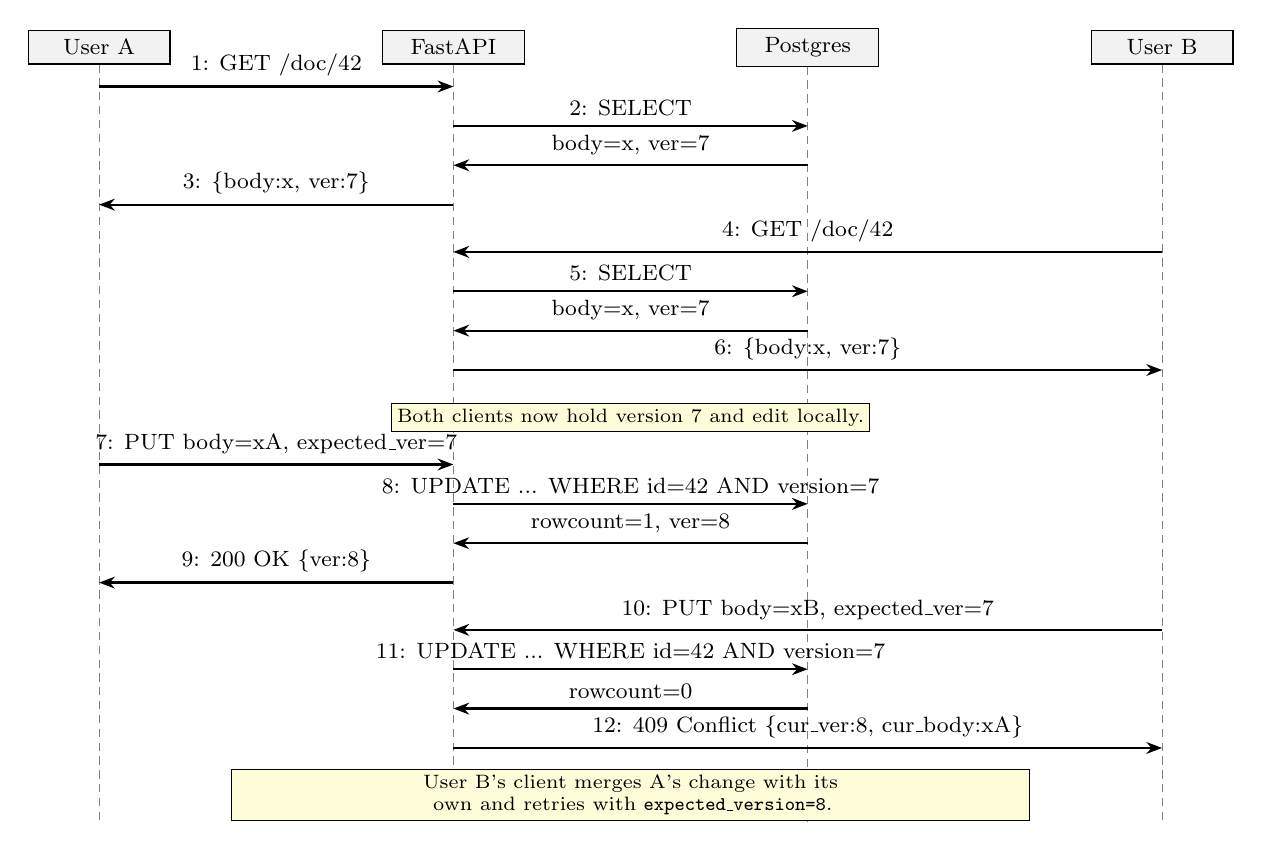
\begin{tikzpicture}[
    >={Stealth[length=2mm]},
    font=\footnotesize,
    actor/.style={draw, fill=gray!10, minimum width=18mm, minimum height=4mm},
    note/.style={draw, fill=yellow!15, font=\scriptsize, inner sep=2pt},
    msg/.style={->, thick}
]
% lifelines
\node[actor] (A)   at (0, 0)    {User A};
\node[actor] (API) at (4.5, 0)  {FastAPI};
\node[actor] (DB)  at (9, 0)    {Postgres};
\node[actor] (B)   at (13.5, 0) {User B};

\foreach \n in {A, API, DB, B} {
    \draw[densely dashed, gray] (\n.south) -- ++(0,-9.6);
}

% step counter (we'll just use small numbers)
% A reads
\draw[msg] (0, -0.5)  -- node[above]{1: GET /doc/42}        (4.5, -0.5);
\draw[msg] (4.5, -1)  -- node[above]{2: SELECT}             (9, -1);
\draw[msg] (9, -1.5)  -- node[above]{body=x, ver=7}         (4.5, -1.5);
\draw[msg] (4.5, -2)  -- node[above]{3: \{body:x, ver:7\}}  (0, -2);

% B reads
\draw[msg] (13.5, -2.6) -- node[above]{4: GET /doc/42}      (4.5, -2.6);
\draw[msg] (4.5, -3.1)  -- node[above]{5: SELECT}           (9, -3.1);
\draw[msg] (9, -3.6)    -- node[above]{body=x, ver=7}       (4.5, -3.6);
\draw[msg] (4.5, -4.1)  -- node[above]{6: \{body:x, ver:7\}}(13.5, -4.1);

\node[note] at (6.75, -4.7) {Both clients now hold version 7 and edit locally.};

% A writes -> ok
\draw[msg] (0, -5.3)  -- node[above]{7: PUT body=xA, expected\_ver=7} (4.5, -5.3);
\draw[msg] (4.5, -5.8) -- node[above]{8: UPDATE ... WHERE id=42 AND version=7} (9, -5.8);
\draw[msg] (9, -6.3)  -- node[above]{rowcount=1, ver=8}    (4.5, -6.3);
\draw[msg] (4.5, -6.8) -- node[above]{9: 200 OK \{ver:8\}} (0, -6.8);

% B writes -> conflict
\draw[msg] (13.5, -7.4) -- node[above]{10: PUT body=xB, expected\_ver=7} (4.5, -7.4);
\draw[msg] (4.5, -7.9)  -- node[above]{11: UPDATE ... WHERE id=42 AND version=7} (9, -7.9);
\draw[msg] (9, -8.4)    -- node[above]{rowcount=0}          (4.5, -8.4);
\draw[msg] (4.5, -8.9)  -- node[above]{12: 409 Conflict \{cur\_ver:8, cur\_body:xA\}} (13.5, -8.9);

\node[note, text width=10cm, align=center] at (6.75, -9.5)
    {User B's client merges A's change with its own and retries with \texttt{expected\_version=8}.};
\end{tikzpicture}
\end{center}

\subsection*{2.2 Coordination --- idempotent webhooks with a durable inbox + DLQ}
\begin{itemize}
  \item \textbf{Idempotency key.} Persist Clerk's \texttt{event.id} in a unique-indexed \texttt{webhook\_inbox}
  \emph{before} any business logic. A duplicate insert returns 200 immediately --- safe under at-least-once retries.
  \item \textbf{Outbox pattern (receiver-side).} The handler inserts into \texttt{webhook\_inbox} and into a
  \texttt{pending\_events} queue in one DB transaction. A background worker drains the queue and performs the
  side effect, so neither the inbox row nor the effect can exist without the other.
  \item \textbf{Retries with exponential backoff} (1s, 5s, 25s, 2m, 10m). The HTTP handler returns in \(<\)200 ms.
  \item \textbf{Dead-letter queue.} After $N$ failed retries the row moves to \texttt{dead\_letter\_events} and a
  Slack/PagerDuty alert fires --- we never silently drop a cancellation.
  \item \textbf{Monotonic ordering.} Compare each event's Clerk timestamp against
  \texttt{users.last\_clerk\_event\_at} and discard older events; this fixes out-of-order
  \texttt{created}/\texttt{deleted}.
\end{itemize}

\subsection*{2.3 Fault Tolerance --- Circuit Breaker + Fallback (the implemented fix)}
Wrap every LLM call in a three-state breaker --- \texttt{CLOSED}, \texttt{OPEN}, \texttt{HALF\_OPEN} --- with a strict
per-call timeout (e.g.\ 2 s, far below the 60 s upstream hang).
\begin{itemize}
  \item \textbf{CLOSED} --- calls flow through; consecutive failures are counted.
  \item \textbf{OPEN} --- once \texttt{failure\_threshold} is hit, every call is short-circuited and the fallback is
  returned in microseconds. The sick upstream gets air to recover and our worker pool is no longer starved.
  \item \textbf{HALF\_OPEN} --- after \texttt{recovery\_timeout} seconds, exactly one probe call is allowed through.
  Success $\rightarrow$ \texttt{CLOSED}. Failure $\rightarrow$ \texttt{OPEN} for another window.
\end{itemize}
The \textbf{fallback} is the second half of the pattern: instead of HTTP 500 we serve a degraded-but-correct response
(a cached study tip / last-known answer) tagged with \texttt{fallback:true} so the UI can show a banner. This is
implemented in \texttt{app/circuit\_breaker.py} and exercised by \texttt{pytest -v}.

\subsection*{2.4 CAP trade-offs}
CAP forces us to pick two of \{Consistency, Availability, Partition-tolerance\}. On a real WAN we always have
Partition-tolerance, so each design picks \textbf{C} or \textbf{A} --- and the third axis we tune is latency.

\begin{center}
\footnotesize
\begin{tabular}{@{}lll p{8.0cm}@{}}
\toprule
\textbf{Sub-system} & \textbf{Pattern} & \textbf{Choice} & \textbf{Why} \\
\midrule
Document edits      & Optimistic Locking      & \textbf{CP}                    & A stale write is rejected (409). We sacrifice write-availability during a conflict to preserve correctness --- losing user work is unacceptable. \\
\addlinespace
Webhook handling    & Idempotent inbox + DLQ  & \textbf{AP, eventually consistent} & The endpoint always returns 200 fast (A), but the \texttt{is\_premium} flag may lag the event by seconds while the worker drains. \\
\addlinespace
LLM tutor           & Circuit Breaker + fallback & \textbf{AP}                 & The fallback is not the freshest LLM output, so we trade content-consistency for API availability. Latency improves dramatically: a 60 s hang becomes a sub-millisecond fallback. \\
\bottomrule
\end{tabular}
\end{center}

The system is deliberately \textbf{mixed-consistency}: strong where data loss is unacceptable (documents), eventually
consistent where unavailability would be more harmful than a few seconds of staleness (subscription state, AI answers).

\end{document}
